% Created by tikzDevice version 0.10.1 on 2017-10-30 17:28:36
% !TEX encoding = UTF-8 Unicode
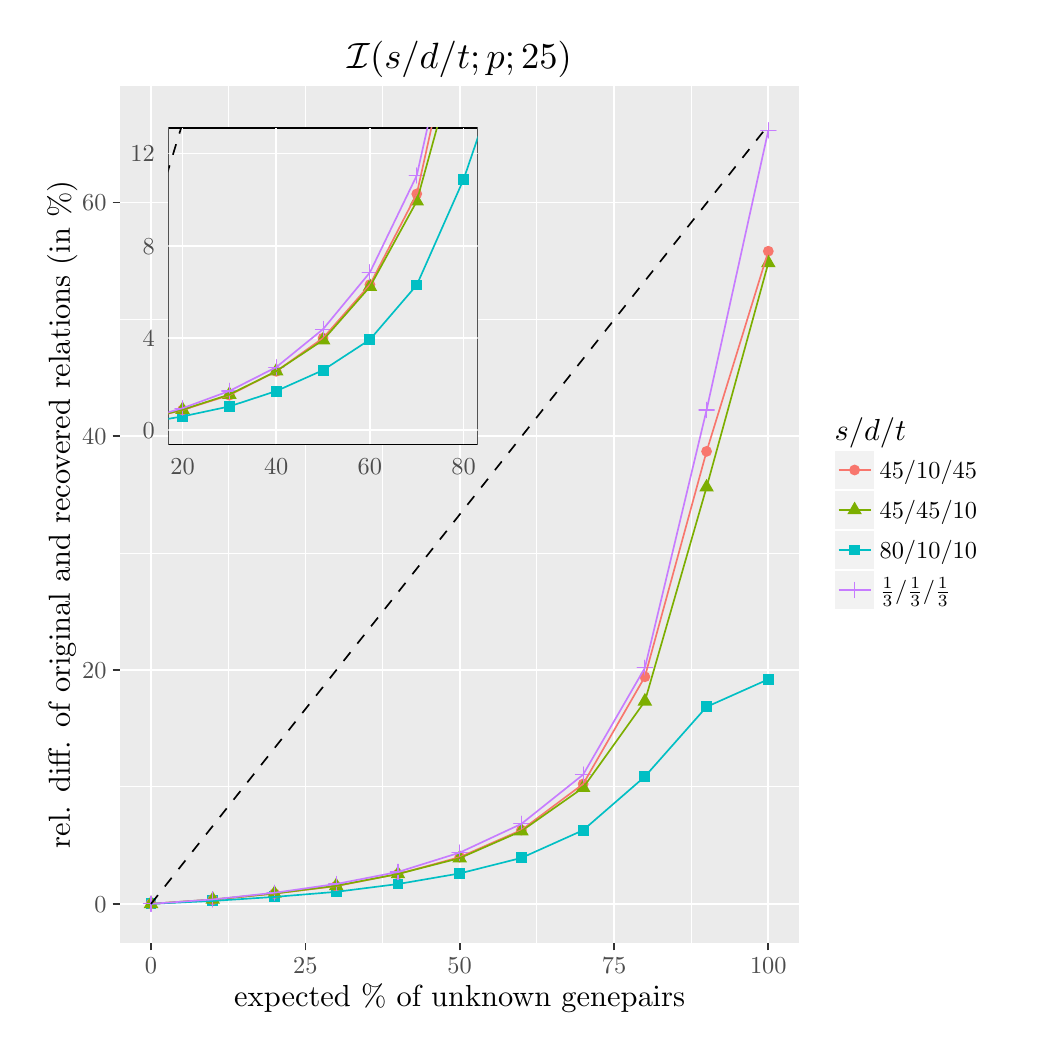
\begin{tikzpicture}[x=1pt,y=1pt]
\definecolor{fillColor}{RGB}{255,255,255}
\path[use as bounding box,fill=fillColor,fill opacity=0.00] (0,0) rectangle (361.35,361.35);
\begin{scope}
\path[clip] (  0.00,  0.00) rectangle (361.35,361.35);
\definecolor{drawColor}{RGB}{255,255,255}
\definecolor{fillColor}{RGB}{255,255,255}

\path[draw=drawColor,line width= 0.6pt,line join=round,line cap=round,fill=fillColor] (  0.00,  0.00) rectangle (361.35,361.35);
\end{scope}
\begin{scope}
\path[clip] ( 33.42, 30.69) rectangle (278.78,340.16);
\definecolor{fillColor}{gray}{0.92}

\path[fill=fillColor] ( 33.42, 30.69) rectangle (278.78,340.16);
\definecolor{drawColor}{RGB}{255,255,255}

\path[draw=drawColor,line width= 0.3pt,line join=round] ( 33.42, 87.00) --
	(278.78, 87.00);

\path[draw=drawColor,line width= 0.3pt,line join=round] ( 33.42,171.48) --
	(278.78,171.48);

\path[draw=drawColor,line width= 0.3pt,line join=round] ( 33.42,255.97) --
	(278.78,255.97);

\path[draw=drawColor,line width= 0.3pt,line join=round] ( 72.46, 30.69) --
	( 72.46,340.16);

\path[draw=drawColor,line width= 0.3pt,line join=round] (128.22, 30.69) --
	(128.22,340.16);

\path[draw=drawColor,line width= 0.3pt,line join=round] (183.98, 30.69) --
	(183.98,340.16);

\path[draw=drawColor,line width= 0.3pt,line join=round] (239.75, 30.69) --
	(239.75,340.16);

\path[draw=drawColor,line width= 0.6pt,line join=round] ( 33.42, 44.75) --
	(278.78, 44.75);

\path[draw=drawColor,line width= 0.6pt,line join=round] ( 33.42,129.24) --
	(278.78,129.24);

\path[draw=drawColor,line width= 0.6pt,line join=round] ( 33.42,213.73) --
	(278.78,213.73);

\path[draw=drawColor,line width= 0.6pt,line join=round] ( 33.42,298.21) --
	(278.78,298.21);

\path[draw=drawColor,line width= 0.6pt,line join=round] ( 44.58, 30.69) --
	( 44.58,340.16);

\path[draw=drawColor,line width= 0.6pt,line join=round] (100.34, 30.69) --
	(100.34,340.16);

\path[draw=drawColor,line width= 0.6pt,line join=round] (156.10, 30.69) --
	(156.10,340.16);

\path[draw=drawColor,line width= 0.6pt,line join=round] (211.87, 30.69) --
	(211.87,340.16);

\path[draw=drawColor,line width= 0.6pt,line join=round] (267.63, 30.69) --
	(267.63,340.16);
\definecolor{fillColor}{RGB}{0,191,196}

\path[fill=fillColor] ( 42.61, 42.79) --
	( 46.54, 42.79) --
	( 46.54, 46.72) --
	( 42.61, 46.72) --
	cycle;

\path[fill=fillColor] ( 64.92, 43.84) --
	( 68.84, 43.84) --
	( 68.84, 47.76) --
	( 64.92, 47.76) --
	cycle;

\path[fill=fillColor] ( 87.22, 45.29) --
	( 91.15, 45.29) --
	( 91.15, 49.21) --
	( 87.22, 49.21) --
	cycle;

\path[fill=fillColor] (109.53, 47.12) --
	(113.45, 47.12) --
	(113.45, 51.04) --
	(109.53, 51.04) --
	cycle;

\path[fill=fillColor] (131.84, 49.93) --
	(135.76, 49.93) --
	(135.76, 53.86) --
	(131.84, 53.86) --
	cycle;

\path[fill=fillColor] (154.14, 53.77) --
	(158.06, 53.77) --
	(158.06, 57.69) --
	(154.14, 57.69) --
	cycle;

\path[fill=fillColor] (176.45, 59.38) --
	(180.37, 59.38) --
	(180.37, 63.30) --
	(176.45, 63.30) --
	cycle;

\path[fill=fillColor] (198.75, 69.39) --
	(202.68, 69.39) --
	(202.68, 73.31) --
	(198.75, 73.31) --
	cycle;

\path[fill=fillColor] (221.06, 88.77) --
	(224.98, 88.77) --
	(224.98, 92.69) --
	(221.06, 92.69) --
	cycle;

\path[fill=fillColor] (243.36,113.97) --
	(247.29,113.97) --
	(247.29,117.89) --
	(243.36,117.89) --
	cycle;

\path[fill=fillColor] (265.67,123.92) --
	(269.59,123.92) --
	(269.59,127.84) --
	(265.67,127.84) --
	cycle;
\definecolor{fillColor}{RGB}{248,118,109}

\path[fill=fillColor] ( 44.58, 44.75) circle (  1.96);

\path[fill=fillColor] ( 66.88, 46.23) circle (  1.96);

\path[fill=fillColor] ( 89.19, 48.44) circle (  1.96);

\path[fill=fillColor] (111.49, 51.15) circle (  1.96);

\path[fill=fillColor] (133.80, 55.52) circle (  1.96);

\path[fill=fillColor] (156.10, 61.62) circle (  1.96);

\path[fill=fillColor] (178.41, 71.42) circle (  1.96);

\path[fill=fillColor] (200.71, 88.05) circle (  1.96);

\path[fill=fillColor] (223.02,126.79) circle (  1.96);

\path[fill=fillColor] (245.32,208.24) circle (  1.96);

\path[fill=fillColor] (267.63,280.57) circle (  1.96);
\definecolor{fillColor}{RGB}{124,174,0}

\path[fill=fillColor] ( 44.58, 47.80) --
	( 47.22, 43.23) --
	( 41.93, 43.23) --
	cycle;

\path[fill=fillColor] ( 66.88, 49.36) --
	( 69.52, 44.78) --
	( 64.24, 44.78) --
	cycle;

\path[fill=fillColor] ( 89.19, 51.54) --
	( 91.83, 46.96) --
	( 86.54, 46.96) --
	cycle;

\path[fill=fillColor] (111.49, 54.31) --
	(114.13, 49.73) --
	(108.85, 49.73) --
	cycle;

\path[fill=fillColor] (133.80, 58.58) --
	(136.44, 54.00) --
	(131.15, 54.00) --
	cycle;

\path[fill=fillColor] (156.10, 64.31) --
	(158.75, 59.73) --
	(153.46, 59.73) --
	cycle;

\path[fill=fillColor] (178.41, 74.08) --
	(181.05, 69.50) --
	(175.77, 69.50) --
	cycle;

\path[fill=fillColor] (200.71, 89.75) --
	(203.36, 85.18) --
	(198.07, 85.18) --
	cycle;

\path[fill=fillColor] (223.02,120.97) --
	(225.66,116.40) --
	(220.38,116.40) --
	cycle;

\path[fill=fillColor] (245.32,198.33) --
	(247.97,193.75) --
	(242.68,193.75) --
	cycle;

\path[fill=fillColor] (267.63,279.37) --
	(270.27,274.79) --
	(264.99,274.79) --
	cycle;
\definecolor{drawColor}{RGB}{199,124,255}

\path[draw=drawColor,line width= 0.4pt,line join=round,line cap=round] ( 41.80, 44.75) -- ( 47.35, 44.75);

\path[draw=drawColor,line width= 0.4pt,line join=round,line cap=round] ( 44.58, 41.98) -- ( 44.58, 47.53);

\path[draw=drawColor,line width= 0.4pt,line join=round,line cap=round] ( 64.11, 46.34) -- ( 69.66, 46.34);

\path[draw=drawColor,line width= 0.4pt,line join=round,line cap=round] ( 66.88, 43.56) -- ( 66.88, 49.11);

\path[draw=drawColor,line width= 0.4pt,line join=round,line cap=round] ( 86.41, 48.75) -- ( 91.96, 48.75);

\path[draw=drawColor,line width= 0.4pt,line join=round,line cap=round] ( 89.19, 45.98) -- ( 89.19, 51.53);

\path[draw=drawColor,line width= 0.4pt,line join=round,line cap=round] (108.72, 51.92) -- (114.27, 51.92);

\path[draw=drawColor,line width= 0.4pt,line join=round,line cap=round] (111.49, 49.14) -- (111.49, 54.69);

\path[draw=drawColor,line width= 0.4pt,line join=round,line cap=round] (131.02, 56.27) -- (136.57, 56.27);

\path[draw=drawColor,line width= 0.4pt,line join=round,line cap=round] (133.80, 53.50) -- (133.80, 59.05);

\path[draw=drawColor,line width= 0.4pt,line join=round,line cap=round] (153.33, 63.25) -- (158.88, 63.25);

\path[draw=drawColor,line width= 0.4pt,line join=round,line cap=round] (156.10, 60.48) -- (156.10, 66.03);

\path[draw=drawColor,line width= 0.4pt,line join=round,line cap=round] (175.63, 73.65) -- (181.18, 73.65);

\path[draw=drawColor,line width= 0.4pt,line join=round,line cap=round] (178.41, 70.88) -- (178.41, 76.43);

\path[draw=drawColor,line width= 0.4pt,line join=round,line cap=round] (197.94, 91.43) -- (203.49, 91.43);

\path[draw=drawColor,line width= 0.4pt,line join=round,line cap=round] (200.71, 88.65) -- (200.71, 94.20);

\path[draw=drawColor,line width= 0.4pt,line join=round,line cap=round] (220.24,129.99) -- (225.79,129.99);

\path[draw=drawColor,line width= 0.4pt,line join=round,line cap=round] (223.02,127.22) -- (223.02,132.77);

\path[draw=drawColor,line width= 0.4pt,line join=round,line cap=round] (242.55,223.20) -- (248.10,223.20);

\path[draw=drawColor,line width= 0.4pt,line join=round,line cap=round] (245.32,220.43) -- (245.32,225.98);

\path[draw=drawColor,line width= 0.4pt,line join=round,line cap=round] (264.85,324.22) -- (270.40,324.22);

\path[draw=drawColor,line width= 0.4pt,line join=round,line cap=round] (267.63,321.44) -- (267.63,326.99);
\definecolor{drawColor}{RGB}{248,118,109}

\path[draw=drawColor,line width= 0.6pt,line join=round] ( 44.58, 44.75) --
	( 66.88, 46.23) --
	( 89.19, 48.44) --
	(111.49, 51.15) --
	(133.80, 55.52) --
	(156.10, 61.62) --
	(178.41, 71.42) --
	(200.71, 88.05) --
	(223.02,126.79) --
	(245.32,208.24) --
	(267.63,280.57);
\definecolor{drawColor}{RGB}{124,174,0}

\path[draw=drawColor,line width= 0.6pt,line join=round] ( 44.58, 44.75) --
	( 66.88, 46.31) --
	( 89.19, 48.49) --
	(111.49, 51.26) --
	(133.80, 55.53) --
	(156.10, 61.25) --
	(178.41, 71.03) --
	(200.71, 86.70) --
	(223.02,117.92) --
	(245.32,195.28) --
	(267.63,276.32);
\definecolor{drawColor}{RGB}{0,191,196}

\path[draw=drawColor,line width= 0.6pt,line join=round] ( 44.58, 44.75) --
	( 66.88, 45.80) --
	( 89.19, 47.25) --
	(111.49, 49.08) --
	(133.80, 51.90) --
	(156.10, 55.73) --
	(178.41, 61.34) --
	(200.71, 71.35) --
	(223.02, 90.73) --
	(245.32,115.93) --
	(267.63,125.88);
\definecolor{drawColor}{RGB}{199,124,255}

\path[draw=drawColor,line width= 0.6pt,line join=round] ( 44.58, 44.75) --
	( 66.88, 46.34) --
	( 89.19, 48.75) --
	(111.49, 51.92) --
	(133.80, 56.27) --
	(156.10, 63.25) --
	(178.41, 73.65) --
	(200.71, 91.43) --
	(223.02,129.99) --
	(245.32,223.20) --
	(267.63,324.22);
\definecolor{drawColor}{RGB}{0,0,0}

\path[draw=drawColor,line width= 0.6pt,dash pattern=on 4pt off 4pt ,line join=round] ( 44.58, 44.75) --
	( 55.73, 58.82) --
	( 66.88, 72.89) --
	( 78.03, 86.95) --
	( 89.19,101.02) --
	(100.34,115.09) --
	(111.49,129.16) --
	(122.64,143.22) --
	(133.80,157.29) --
	(144.95,171.36) --
	(156.10,185.42) --
	(167.26,199.49) --
	(178.41,213.56) --
	(189.56,227.62) --
	(200.71,241.69) --
	(211.87,255.76) --
	(223.02,269.82) --
	(234.17,283.89) --
	(245.32,297.96) --
	(256.48,312.03) --
	(267.63,326.09);
\end{scope}
\begin{scope}
\path[clip] (  0.00,  0.00) rectangle (361.35,361.35);
\definecolor{drawColor}{gray}{0.30}

\node[text=drawColor,anchor=base east,inner sep=0pt, outer sep=0pt, scale=  0.88] at ( 28.47, 41.72) {0};

\node[text=drawColor,anchor=base east,inner sep=0pt, outer sep=0pt, scale=  0.88] at ( 28.47,126.21) {20};

\node[text=drawColor,anchor=base east,inner sep=0pt, outer sep=0pt, scale=  0.88] at ( 28.47,210.70) {40};

\node[text=drawColor,anchor=base east,inner sep=0pt, outer sep=0pt, scale=  0.88] at ( 28.47,295.18) {60};
\end{scope}
\begin{scope}
\path[clip] (  0.00,  0.00) rectangle (361.35,361.35);
\definecolor{drawColor}{gray}{0.20}

\path[draw=drawColor,line width= 0.6pt,line join=round] ( 30.67, 44.75) --
	( 33.42, 44.75);

\path[draw=drawColor,line width= 0.6pt,line join=round] ( 30.67,129.24) --
	( 33.42,129.24);

\path[draw=drawColor,line width= 0.6pt,line join=round] ( 30.67,213.73) --
	( 33.42,213.73);

\path[draw=drawColor,line width= 0.6pt,line join=round] ( 30.67,298.21) --
	( 33.42,298.21);
\end{scope}
\begin{scope}
\path[clip] (  0.00,  0.00) rectangle (361.35,361.35);
\definecolor{drawColor}{gray}{0.20}

\path[draw=drawColor,line width= 0.6pt,line join=round] ( 44.58, 27.94) --
	( 44.58, 30.69);

\path[draw=drawColor,line width= 0.6pt,line join=round] (100.34, 27.94) --
	(100.34, 30.69);

\path[draw=drawColor,line width= 0.6pt,line join=round] (156.10, 27.94) --
	(156.10, 30.69);

\path[draw=drawColor,line width= 0.6pt,line join=round] (211.87, 27.94) --
	(211.87, 30.69);

\path[draw=drawColor,line width= 0.6pt,line join=round] (267.63, 27.94) --
	(267.63, 30.69);
\end{scope}
\begin{scope}
\path[clip] (  0.00,  0.00) rectangle (361.35,361.35);
\definecolor{drawColor}{gray}{0.30}

\node[text=drawColor,anchor=base,inner sep=0pt, outer sep=0pt, scale=  0.88] at ( 44.58, 19.68) {0};

\node[text=drawColor,anchor=base,inner sep=0pt, outer sep=0pt, scale=  0.88] at (100.34, 19.68) {25};

\node[text=drawColor,anchor=base,inner sep=0pt, outer sep=0pt, scale=  0.88] at (156.10, 19.68) {50};

\node[text=drawColor,anchor=base,inner sep=0pt, outer sep=0pt, scale=  0.88] at (211.87, 19.68) {75};

\node[text=drawColor,anchor=base,inner sep=0pt, outer sep=0pt, scale=  0.88] at (267.63, 19.68) {100};
\end{scope}
\begin{scope}
\path[clip] (  0.00,  0.00) rectangle (361.35,361.35);
\definecolor{drawColor}{RGB}{0,0,0}

\node[text=drawColor,anchor=base,inner sep=0pt, outer sep=0pt, scale=  1.10] at (156.10,  7.70) {expected \% of unknown genepairs};
\end{scope}
\begin{scope}
\path[clip] (  0.00,  0.00) rectangle (361.35,361.35);
\definecolor{drawColor}{RGB}{0,0,0}

\node[text=drawColor,rotate= 90.00,anchor=base,inner sep=0pt, outer sep=0pt, scale=  1.10] at ( 15.28,185.42) {rel. diff. of original and recovered relations (in \%)};
\end{scope}
\begin{scope}
\path[clip] (  0.00,  0.00) rectangle (361.35,361.35);
\definecolor{fillColor}{RGB}{255,255,255}

\path[fill=fillColor] (287.32,146.65) rectangle (347.31,224.19);
\end{scope}
\begin{scope}
\path[clip] (  0.00,  0.00) rectangle (361.35,361.35);
\definecolor{drawColor}{RGB}{0,0,0}

\node[text=drawColor,anchor=base west,inner sep=0pt, outer sep=0pt, scale=  1.10] at (291.59,212.35) {$\mathfrak{s}/\mathfrak{d}/\mathfrak{t}$};
\end{scope}
\begin{scope}
\path[clip] (  0.00,  0.00) rectangle (361.35,361.35);
\definecolor{drawColor}{RGB}{255,255,255}
\definecolor{fillColor}{gray}{0.95}

\path[draw=drawColor,line width= 0.6pt,line join=round,line cap=round,fill=fillColor] (291.59,194.28) rectangle (306.04,208.74);
\end{scope}
\begin{scope}
\path[clip] (  0.00,  0.00) rectangle (361.35,361.35);
\definecolor{fillColor}{RGB}{248,118,109}

\path[fill=fillColor] (298.81,201.51) circle (  1.96);
\end{scope}
\begin{scope}
\path[clip] (  0.00,  0.00) rectangle (361.35,361.35);
\definecolor{drawColor}{RGB}{248,118,109}

\path[draw=drawColor,line width= 0.6pt,line join=round] (293.03,201.51) -- (304.59,201.51);
\end{scope}
\begin{scope}
\path[clip] (  0.00,  0.00) rectangle (361.35,361.35);
\definecolor{drawColor}{RGB}{255,255,255}
\definecolor{fillColor}{gray}{0.95}

\path[draw=drawColor,line width= 0.6pt,line join=round,line cap=round,fill=fillColor] (291.59,179.83) rectangle (306.04,194.28);
\end{scope}
\begin{scope}
\path[clip] (  0.00,  0.00) rectangle (361.35,361.35);
\definecolor{fillColor}{RGB}{124,174,0}

\path[fill=fillColor] (298.81,190.11) --
	(301.45,185.53) --
	(296.17,185.53) --
	cycle;
\end{scope}
\begin{scope}
\path[clip] (  0.00,  0.00) rectangle (361.35,361.35);
\definecolor{drawColor}{RGB}{124,174,0}

\path[draw=drawColor,line width= 0.6pt,line join=round] (293.03,187.06) -- (304.59,187.06);
\end{scope}
\begin{scope}
\path[clip] (  0.00,  0.00) rectangle (361.35,361.35);
\definecolor{drawColor}{RGB}{255,255,255}
\definecolor{fillColor}{gray}{0.95}

\path[draw=drawColor,line width= 0.6pt,line join=round,line cap=round,fill=fillColor] (291.59,165.37) rectangle (306.04,179.83);
\end{scope}
\begin{scope}
\path[clip] (  0.00,  0.00) rectangle (361.35,361.35);
\definecolor{fillColor}{RGB}{0,191,196}

\path[fill=fillColor] (296.85,170.64) --
	(300.77,170.64) --
	(300.77,174.56) --
	(296.85,174.56) --
	cycle;
\end{scope}
\begin{scope}
\path[clip] (  0.00,  0.00) rectangle (361.35,361.35);
\definecolor{drawColor}{RGB}{0,191,196}

\path[draw=drawColor,line width= 0.6pt,line join=round] (293.03,172.60) -- (304.59,172.60);
\end{scope}
\begin{scope}
\path[clip] (  0.00,  0.00) rectangle (361.35,361.35);
\definecolor{drawColor}{RGB}{255,255,255}
\definecolor{fillColor}{gray}{0.95}

\path[draw=drawColor,line width= 0.6pt,line join=round,line cap=round,fill=fillColor] (291.59,150.92) rectangle (306.04,165.37);
\end{scope}
\begin{scope}
\path[clip] (  0.00,  0.00) rectangle (361.35,361.35);
\definecolor{drawColor}{RGB}{199,124,255}

\path[draw=drawColor,line width= 0.4pt,line join=round,line cap=round] (296.04,158.15) -- (301.59,158.15);

\path[draw=drawColor,line width= 0.4pt,line join=round,line cap=round] (298.81,155.37) -- (298.81,160.92);
\end{scope}
\begin{scope}
\path[clip] (  0.00,  0.00) rectangle (361.35,361.35);
\definecolor{drawColor}{RGB}{199,124,255}

\path[draw=drawColor,line width= 0.6pt,line join=round] (293.03,158.15) -- (304.59,158.15);
\end{scope}
\begin{scope}
\path[clip] (  0.00,  0.00) rectangle (361.35,361.35);
\definecolor{drawColor}{RGB}{0,0,0}

\node[text=drawColor,anchor=base west,inner sep=0pt, outer sep=0pt, scale=  0.88] at (307.85,198.48) {$45/10/45$};
\end{scope}
\begin{scope}
\path[clip] (  0.00,  0.00) rectangle (361.35,361.35);
\definecolor{drawColor}{RGB}{0,0,0}

\node[text=drawColor,anchor=base west,inner sep=0pt, outer sep=0pt, scale=  0.88] at (307.85,184.02) {$45/45/10$};
\end{scope}
\begin{scope}
\path[clip] (  0.00,  0.00) rectangle (361.35,361.35);
\definecolor{drawColor}{RGB}{0,0,0}

\node[text=drawColor,anchor=base west,inner sep=0pt, outer sep=0pt, scale=  0.88] at (307.85,169.57) {$80/10/10$};
\end{scope}
\begin{scope}
\path[clip] (  0.00,  0.00) rectangle (361.35,361.35);
\definecolor{drawColor}{RGB}{0,0,0}

\node[text=drawColor,anchor=base west,inner sep=0pt, outer sep=0pt, scale=  0.88] at (307.85,155.12) {$\frac{1}{3}/\frac{1}{3}/\frac{1}{3}$};
\end{scope}
\begin{scope}
\path[clip] (  0.00,  0.00) rectangle (361.35,361.35);
\definecolor{drawColor}{RGB}{0,0,0}

\node[text=drawColor,anchor=base,inner sep=0pt, outer sep=0pt, scale=  1.32] at (156.10,346.76) {$\mathcal{I}(\mathfrak{s}/\mathfrak{d}/\mathfrak{t};p;25)$};
\end{scope}
\begin{scope}
\path[clip] ( 54.20,216.81) rectangle (162.61,325.21);
\definecolor{drawColor}{RGB}{255,255,255}
\definecolor{fillColor}{RGB}{255,255,255}

\path[draw=drawColor,line width= 0.6pt,line join=round,line cap=round,fill=fillColor] ( 54.20,216.81) rectangle (162.61,325.21);
\end{scope}
\begin{scope}
\path[clip] ( 50.88,210.75) rectangle (162.61,325.21);
\definecolor{drawColor}{RGB}{0,0,0}
\definecolor{fillColor}{gray}{0.92}

\path[draw=drawColor,line width= 0.6pt,line join=round,line cap=round,fill=fillColor] ( 50.88,210.75) rectangle (162.61,325.21);
\definecolor{drawColor}{RGB}{255,255,255}

\path[draw=drawColor,line width= 0.6pt,line join=round] ( 50.88,215.95) --
	(162.61,215.95);

\path[draw=drawColor,line width= 0.6pt,line join=round] ( 50.88,249.25) --
	(162.61,249.25);

\path[draw=drawColor,line width= 0.6pt,line join=round] ( 50.88,282.55) --
	(162.61,282.55);

\path[draw=drawColor,line width= 0.6pt,line join=round] ( 50.88,315.85) --
	(162.61,315.85);

\path[draw=drawColor,line width= 0.6pt,line join=round] ( 55.96,210.75) --
	( 55.96,325.21);

\path[draw=drawColor,line width= 0.6pt,line join=round] ( 89.81,210.75) --
	( 89.81,325.21);

\path[draw=drawColor,line width= 0.6pt,line join=round] (123.67,210.75) --
	(123.67,325.21);

\path[draw=drawColor,line width= 0.6pt,line join=round] (157.53,210.75) --
	(157.53,325.21);
\definecolor{fillColor}{RGB}{0,191,196}

\path[fill=fillColor] ( 20.14,213.99) --
	( 24.06,213.99) --
	( 24.06,217.91) --
	( 20.14,217.91) --
	cycle;

\path[fill=fillColor] ( 37.07,216.05) --
	( 40.99,216.05) --
	( 40.99,219.98) --
	( 37.07,219.98) --
	cycle;

\path[fill=fillColor] ( 54.00,218.91) --
	( 57.92,218.91) --
	( 57.92,222.83) --
	( 54.00,222.83) --
	cycle;

\path[fill=fillColor] ( 70.92,222.52) --
	( 74.85,222.52) --
	( 74.85,226.44) --
	( 70.92,226.44) --
	cycle;

\path[fill=fillColor] ( 87.85,228.06) --
	( 91.78,228.06) --
	( 91.78,231.99) --
	( 87.85,231.99) --
	cycle;

\path[fill=fillColor] (104.78,235.63) --
	(108.71,235.63) --
	(108.71,239.55) --
	(104.78,239.55) --
	cycle;

\path[fill=fillColor] (121.71,246.68) --
	(125.63,246.68) --
	(125.63,250.60) --
	(121.71,250.60) --
	cycle;

\path[fill=fillColor] (138.64,266.40) --
	(142.56,266.40) --
	(142.56,270.32) --
	(138.64,270.32) --
	cycle;

\path[fill=fillColor] (155.57,304.60) --
	(159.49,304.60) --
	(159.49,308.52) --
	(155.57,308.52) --
	cycle;

\path[fill=fillColor] (172.50,354.25) --
	(176.42,354.25) --
	(176.42,358.18) --
	(172.50,358.18) --
	cycle;
\definecolor{fillColor}{RGB}{248,118,109}

\path[fill=fillColor] ( 22.10,215.95) circle (  1.96);

\path[fill=fillColor] ( 39.03,218.85) circle (  1.96);

\path[fill=fillColor] ( 55.96,223.21) circle (  1.96);

\path[fill=fillColor] ( 72.89,228.55) circle (  1.96);

\path[fill=fillColor] ( 89.81,237.17) circle (  1.96);

\path[fill=fillColor] (106.74,249.18) circle (  1.96);

\path[fill=fillColor] (123.67,268.50) circle (  1.96);

\path[fill=fillColor] (140.60,301.28) circle (  1.96);
\definecolor{fillColor}{RGB}{124,174,0}

\path[fill=fillColor] ( 22.10,219.00) --
	( 24.74,214.43) --
	( 19.46,214.43) --
	cycle;

\path[fill=fillColor] ( 39.03,222.07) --
	( 41.67,217.49) --
	( 36.39,217.49) --
	cycle;

\path[fill=fillColor] ( 55.96,226.37) --
	( 58.60,221.79) --
	( 53.31,221.79) --
	cycle;

\path[fill=fillColor] ( 72.89,231.82) --
	( 75.53,227.25) --
	( 70.24,227.25) --
	cycle;

\path[fill=fillColor] ( 89.81,240.24) --
	( 92.46,235.66) --
	( 87.17,235.66) --
	cycle;

\path[fill=fillColor] (106.74,251.52) --
	(109.39,246.94) --
	(104.10,246.94) --
	cycle;

\path[fill=fillColor] (123.67,270.78) --
	(126.31,266.20) --
	(121.03,266.20) --
	cycle;

\path[fill=fillColor] (140.60,301.67) --
	(143.24,297.09) --
	(137.96,297.09) --
	cycle;

\path[fill=fillColor] (158.59,361.35) --
	(160.17,358.62) --
	(154.89,358.62) --
	(156.46,361.35) --
	cycle;
\definecolor{drawColor}{RGB}{199,124,255}

\path[draw=drawColor,line width= 0.4pt,line join=round,line cap=round] ( 19.33,215.95) -- ( 24.87,215.95);

\path[draw=drawColor,line width= 0.4pt,line join=round,line cap=round] ( 22.10,213.18) -- ( 22.10,218.73);

\path[draw=drawColor,line width= 0.4pt,line join=round,line cap=round] ( 36.25,219.07) -- ( 41.80,219.07);

\path[draw=drawColor,line width= 0.4pt,line join=round,line cap=round] ( 39.03,216.30) -- ( 39.03,221.85);

\path[draw=drawColor,line width= 0.4pt,line join=round,line cap=round] ( 53.18,223.83) -- ( 58.73,223.83);

\path[draw=drawColor,line width= 0.4pt,line join=round,line cap=round] ( 55.96,221.06) -- ( 55.96,226.61);

\path[draw=drawColor,line width= 0.4pt,line join=round,line cap=round] ( 70.11,230.07) -- ( 75.66,230.07);

\path[draw=drawColor,line width= 0.4pt,line join=round,line cap=round] ( 72.89,227.30) -- ( 72.89,232.85);

\path[draw=drawColor,line width= 0.4pt,line join=round,line cap=round] ( 87.04,238.65) -- ( 92.59,238.65);

\path[draw=drawColor,line width= 0.4pt,line join=round,line cap=round] ( 89.81,235.88) -- ( 89.81,241.43);

\path[draw=drawColor,line width= 0.4pt,line join=round,line cap=round] (103.97,252.41) -- (109.52,252.41);

\path[draw=drawColor,line width= 0.4pt,line join=round,line cap=round] (106.74,249.64) -- (106.74,255.19);

\path[draw=drawColor,line width= 0.4pt,line join=round,line cap=round] (120.90,272.90) -- (126.45,272.90);

\path[draw=drawColor,line width= 0.4pt,line join=round,line cap=round] (123.67,270.13) -- (123.67,275.68);

\path[draw=drawColor,line width= 0.4pt,line join=round,line cap=round] (137.83,307.93) -- (143.38,307.93);

\path[draw=drawColor,line width= 0.4pt,line join=round,line cap=round] (140.60,305.16) -- (140.60,310.71);
\definecolor{drawColor}{RGB}{248,118,109}

\path[draw=drawColor,line width= 0.6pt,line join=round] ( 22.10,215.95) --
	( 39.03,218.85) --
	( 55.96,223.21) --
	( 72.89,228.55) --
	( 89.81,237.17) --
	(106.74,249.18) --
	(123.67,268.50) --
	(140.60,301.28) --
	(153.92,361.35);
\definecolor{drawColor}{RGB}{124,174,0}

\path[draw=drawColor,line width= 0.6pt,line join=round] ( 22.10,215.95) --
	( 39.03,219.02) --
	( 55.96,223.31) --
	( 72.89,228.77) --
	( 89.81,237.19) --
	(106.74,248.47) --
	(123.67,267.73) --
	(140.60,298.62) --
	(157.53,360.14) --
	(157.66,361.35);
\definecolor{drawColor}{RGB}{0,191,196}

\path[draw=drawColor,line width= 0.6pt,line join=round] ( 22.10,215.95) --
	( 39.03,218.02) --
	( 55.96,220.87) --
	( 72.89,224.48) --
	( 89.81,230.03) --
	(106.74,237.59) --
	(123.67,248.64) --
	(140.60,268.36) --
	(157.53,306.56) --
	(174.46,356.22) --
	(178.89,361.35);
\definecolor{drawColor}{RGB}{199,124,255}

\path[draw=drawColor,line width= 0.6pt,line join=round] ( 22.10,215.95) --
	( 39.03,219.07) --
	( 55.96,223.83) --
	( 72.89,230.07) --
	( 89.81,238.65) --
	(106.74,252.41) --
	(123.67,272.90) --
	(140.60,307.93) --
	(152.50,361.35);
\definecolor{drawColor}{RGB}{0,0,0}

\path[draw=drawColor,line width= 0.6pt,dash pattern=on 4pt off 4pt ,line join=round] ( 22.10,215.95) --
	( 30.56,243.67) --
	( 39.03,271.40) --
	( 47.49,299.12) --
	( 55.96,326.84) --
	( 64.42,354.56) --
	( 66.49,361.35);
\end{scope}
\begin{scope}
\path[clip] (  0.00,  0.00) rectangle (361.35,361.35);
\definecolor{drawColor}{gray}{0.30}

\node[text=drawColor,anchor=base east,inner sep=0pt, outer sep=0pt, scale=  0.88] at ( 45.93,212.92) {0};

\node[text=drawColor,anchor=base east,inner sep=0pt, outer sep=0pt, scale=  0.88] at ( 45.93,246.22) {4};

\node[text=drawColor,anchor=base east,inner sep=0pt, outer sep=0pt, scale=  0.88] at ( 45.93,279.52) {8};

\node[text=drawColor,anchor=base east,inner sep=0pt, outer sep=0pt, scale=  0.88] at ( 45.93,312.82) {12};
\end{scope}
\begin{scope}
\path[clip] (  0.00,  0.00) rectangle (361.35,361.35);
\definecolor{drawColor}{gray}{0.30}

\node[text=drawColor,anchor=base,inner sep=0pt, outer sep=0pt, scale=  0.88] at ( 55.96,199.74) {20};

\node[text=drawColor,anchor=base,inner sep=0pt, outer sep=0pt, scale=  0.88] at ( 89.81,199.74) {40};

\node[text=drawColor,anchor=base,inner sep=0pt, outer sep=0pt, scale=  0.88] at (123.67,199.74) {60};

\node[text=drawColor,anchor=base,inner sep=0pt, outer sep=0pt, scale=  0.88] at (157.53,199.74) {80};
\end{scope}
\end{tikzpicture}
